\chapter{Project Scheduling and Planning}
\label{ch:schedule}

\section{Introduction}
This chapter presents the project schedule, the sequencing of tasks
across the dissertation period (August~2025 -- May~2026) and the
deliverables associated with each phase. The schedule was built using
the Work Breakdown Structure (WBS) approach: the dissertation goal was
decomposed into eleven primary activities organised into five phases,
each with explicit deliverables and an indicative timebox.

\section{Phase-wise Decomposition}

\subsection{Phase 1 -- Planning and Design (Weeks 1--12)}
\begin{itemize}
    \item Literature survey of LLM-based, interactive and multimodal
    storytelling systems.
    \item Requirement analysis with the supervisor: capturing
    functional and non-functional requirements, evaluation criteria.
    \item System design: layered architecture, module boundaries,
    data flow, REST surface, database schema.
\end{itemize}

\subsection{Phase 2 -- Implementation (Weeks 10--23)}
\begin{itemize}
    \item Backend pipeline: seven cooperating Python modules (User
    Input, Context Extraction, Knowledge / Memory, Prompt Engineering,
    Story Generator, Flow Manager, Output Formatter).
    \item LLM provider layer: abstract base class plus concrete
    Ollama, Groq, Hugging Face and OpenAI clients.
    \item Frontend UI development: HTML5/CSS3/Vanilla JS application
    with landing page, single-page question form, story view, admin
    panel and settings panel.
\end{itemize}

\subsection{Phase 3 -- Multimodal Features (Weeks 20--26)}
\begin{itemize}
    \item Image synthesis pipeline integrating Pollinations.ai, with
    sentence-scored prompt extractor and serial throttling queue.
    \item TTS narration via the W3C Web Speech Synthesis interface.
    \item Genre-conditioned ambient music streamed from the SoundHelix
    CDN with fade-in/out crossfades.
    \item D3-based Story Map and Character Relationship Graph
    visualisations.
\end{itemize}

\subsection{Phase 4 -- Evaluation (Weeks 25--29)}
\begin{itemize}
    \item Automated generation of 50 stories across six genres and
    four question budgets; collection of latency, token and
    consistency metrics.
    \item User study with 15 participants producing 30 stories rated
    on 5-point Likert scales across coherence, creativity, engagement
    and consistency.
    \item Consistency-checker evaluation against ground-truth
    annotated segments.
\end{itemize}

\subsection{Phase 5 -- Documentation (Weeks 28--36)}
\begin{itemize}
    \item Dissertation writing covering all chapters of the SAKEC
    project-report format.
    \item Companion IEEE conference-style manuscript suitable for
    submission.
    \item Final review with the supervisor and dissertation defence
    presentation.
\end{itemize}

\section{Gantt Chart}
The full timeline is illustrated in Figure~\ref{fig:gantt}. Tasks
that overlap in time reflect deliberate parallelism: e.g.\ frontend
UI development proceeds alongside backend module work, and multimodal
feature integration overlaps with frontend completion. Colours indicate
the phase to which each task belongs.

\begin{figure}[H]
    \centering
    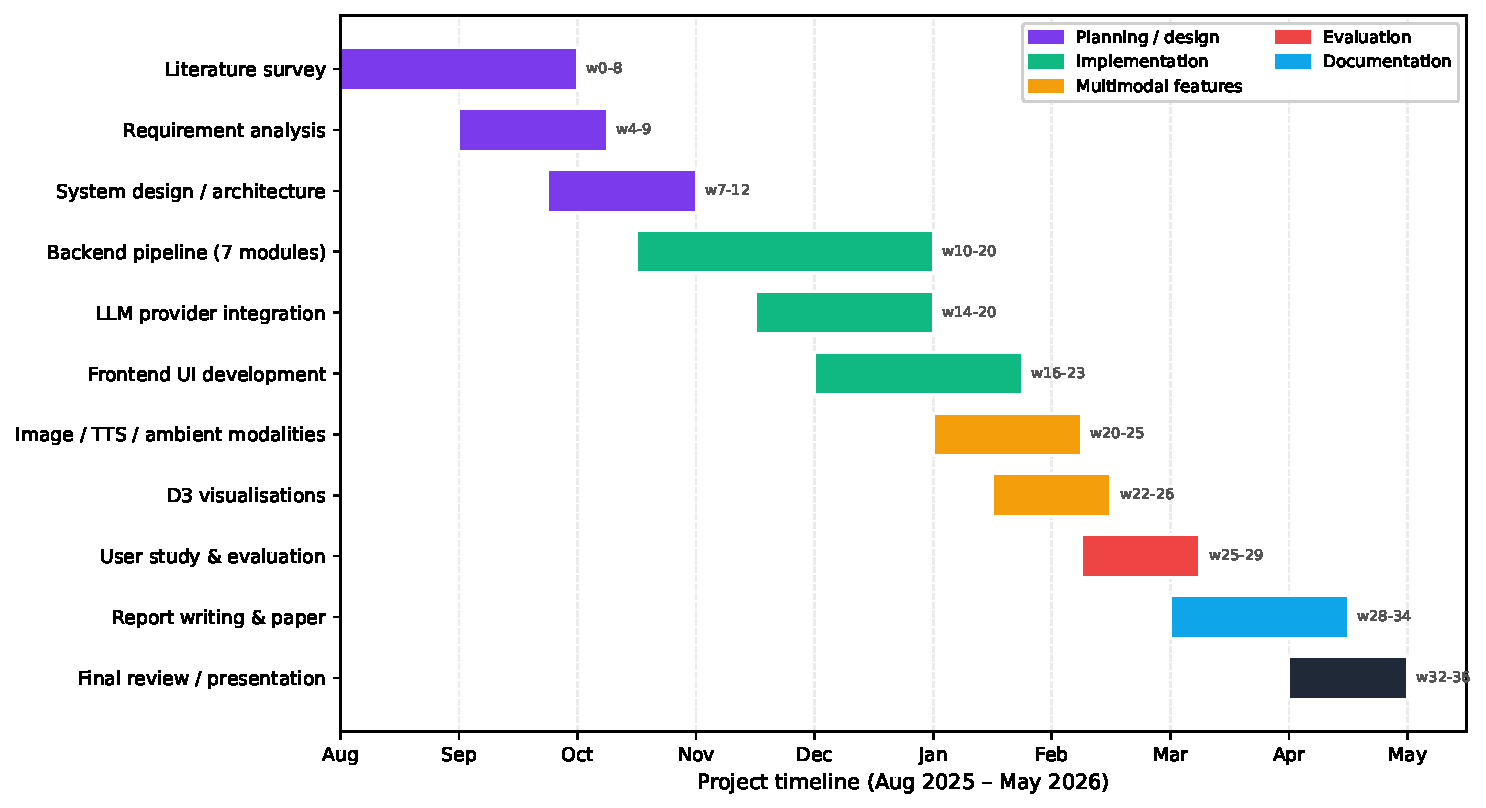
\includegraphics[width=\textwidth]{images/gantt.pdf}
    \caption{Project Gantt chart.}
    \label{fig:gantt}
\end{figure}

\section{Risk and Mitigation Plan}
Table~\ref{tab:risks} lists the principal project risks identified
during planning and the mitigation strategy adopted for each.

\begin{table}[!t]
\caption{Risk register and mitigations.}
\label{tab:risks}
\centering
\renewcommand{\arraystretch}{1.2}
\small
\begin{tabular}{@{}p{4cm} p{3.5cm} p{6cm}@{}}
\toprule
\textbf{Risk} & \textbf{Likelihood / Impact} & \textbf{Mitigation} \\
\midrule
Free-tier image API rate-limits & High / High & Serial throttling queue with 1.2 s spacing and 35 s watchdog. \\
LLM provider downtime           & Medium / Medium & Provider-agnostic abstraction allowing hot-swap via /api/settings. \\
Narrative coherence drift       & Medium / High & Sliding-window context retrieval; consistency checker. \\
Audio autoplay blocked          & High / Low  & Toggle audio on a real user-gesture click; document workaround. \\
User-study schedule slippage    & Medium / Medium & Run rolling sessions across two weeks; remote participation. \\
Cross-origin issues for CDN audio & Medium / Low & Avoid \texttt{crossOrigin="anonymous"}; use plain HTMLAudio. \\
\bottomrule
\end{tabular}
\end{table}

\section{Deliverables}
The principal deliverables tracked across the timeline are:
\begin{itemize}
    \item Open-source codebase released on GitHub
    (\url{https://github.com/DeepPatange/AI-Stroy-Generator}).
    \item This dissertation manuscript prepared in the SAKEC LaTeX
    format.
    \item A companion IEEE-format conference-style research paper.
    \item User-study artefacts: questionnaires, raw ratings, scripts
    for figure generation and statistical reproduction.
    \item Deployable Docker recipe for a single-server demonstration
    environment.
\end{itemize}

\section{Summary}
The schedule was followed substantially as planned. Minor slippages
in the multimodal-features phase --- particularly resolving CORS and
rate-limiting issues for the image API --- were absorbed within the
parallel evaluation window without delaying the dissertation
submission.
